\documentclass{beamer}
%\usepackage{algorithm}
%\usepackage[noend]{algorithmic}
\usepackage{graphicx}

\usetheme[compress]{Dresden}
\setbeamertemplate{navigation symbols}{} 

\title{Locate My Plate \\ A License Plate Localisation System}
\subtitle{presented by: Tjerk Kostelijk, Folkert Huizinga}
\date{}

\begin{document}

\frame{\titlepage}

\setcounter{tocdepth}{1}

\frame
{
  \frametitle{Outline}
  \small
  \tableofcontents
  \normalsize
}

\setcounter{tocdepth}{2}

\section{Introduction}
\frame
{
  \frametitle{Introduction}
	
  \begin{itemize}
  \item <+-| alert@+> blah blah 
  \end{itemize}
}

\section{Results}
\frame
{
  \frametitle{Results}
	\begin{figure}[!ht]
	\centering
	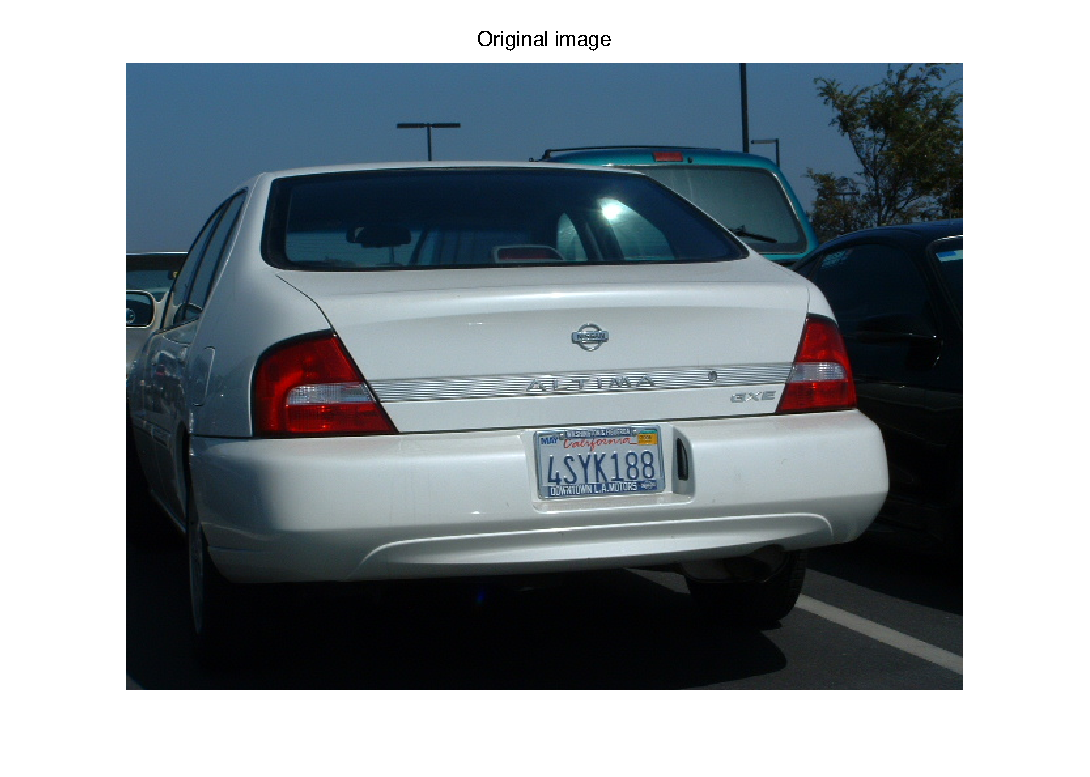
\includegraphics[width=18cm]{../report/img/cascader_original_image}
	\caption{test}
	\label{fig:cascader_original}
	\end{figure}
}


\section{Results}
\frame
{
  \frametitle{Results}
	\begin{figure}[!ht]
	\centering
	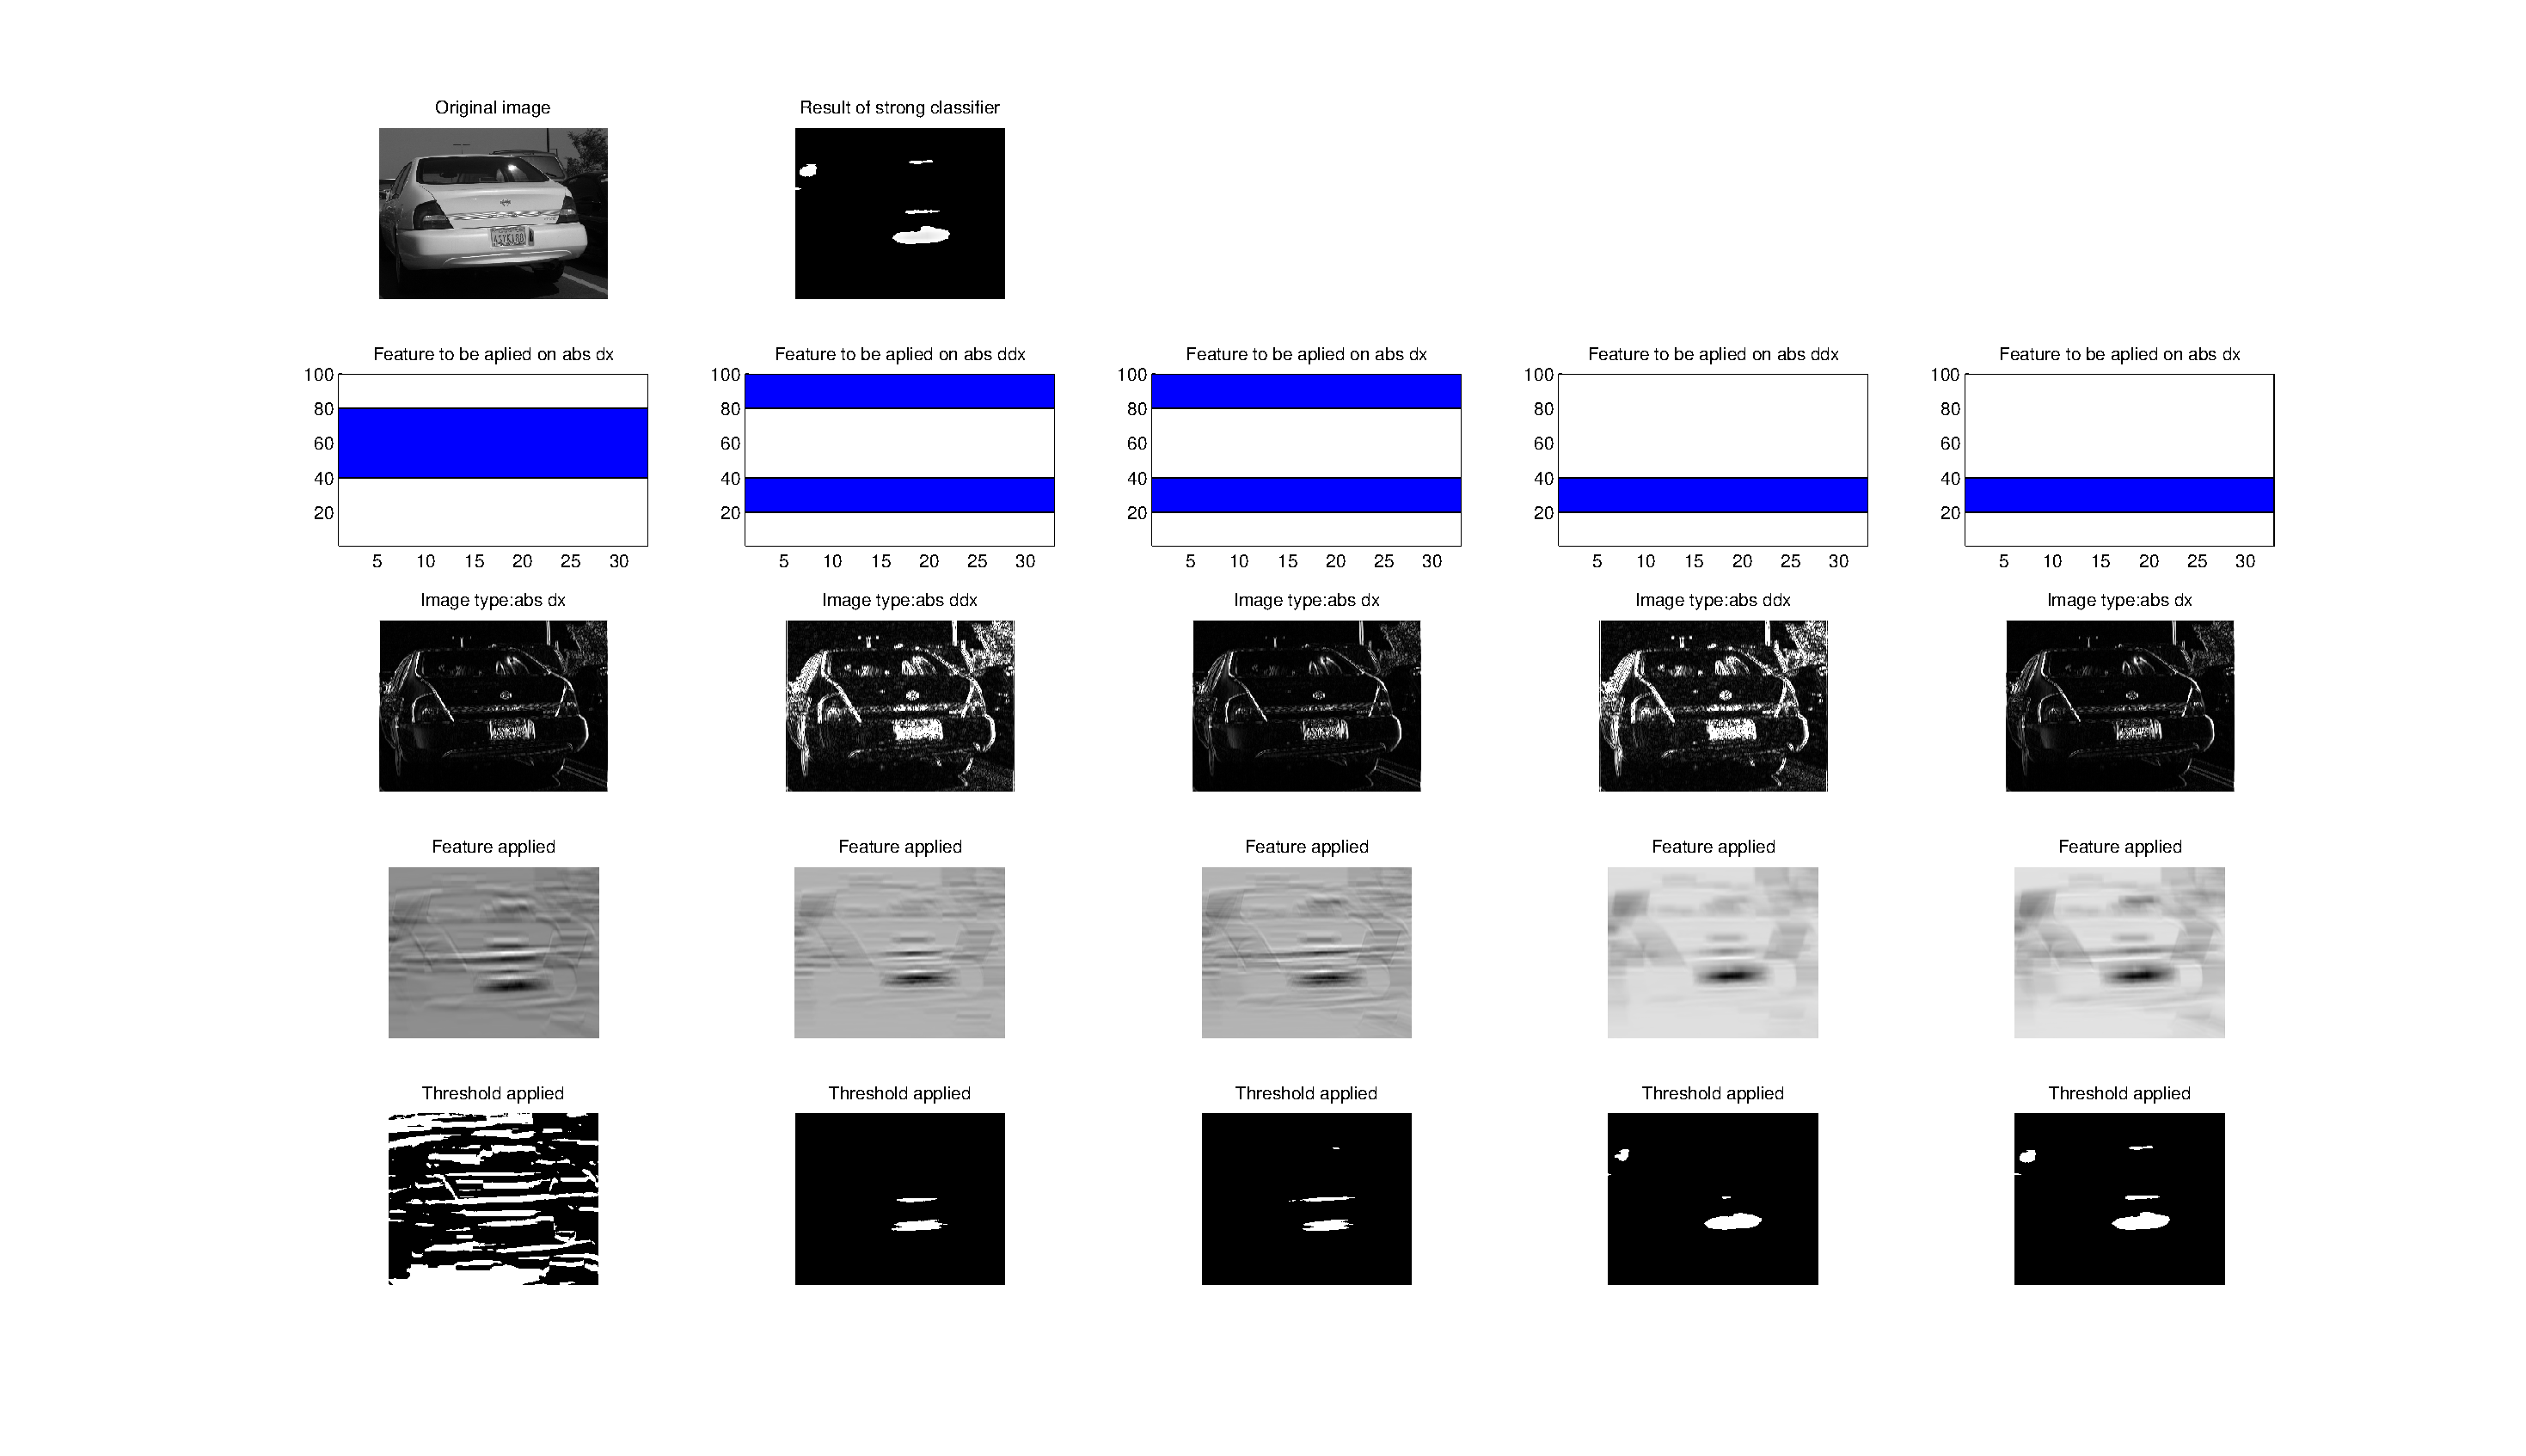
\includegraphics[width=18cm]{../report/img/strongClassifier_layer2_img14}
	\caption{Example of a strongclassifier of a layer with 5 features.}
	\label{fig:strongclassify}
	\end{figure}
}

\AtBeginSection[]
{
 \begin{frame}
  \frametitle{Outline}
  \small
  \tableofcontents[currentsection,hideothersubsections]
  \normalsize
 \end{frame}
}


\end{document}
